% Created 2020-01-10 五 15:24
% Intended LaTeX compiler: pdflatex
\documentclass[11pt]{article}
\usepackage[utf8]{inputenc}
\usepackage[T1]{fontenc}
\usepackage{graphicx}
\usepackage{grffile}
\usepackage{longtable}
\usepackage{wrapfig}
\usepackage{rotating}
\usepackage[normalem]{ulem}
\usepackage{amsmath}
\usepackage{textcomp}
\usepackage{amssymb}
\usepackage{capt-of}
\usepackage{hyperref}
\usepackage{minted}
% TIPS
% \substack{a\\b} for multiple lines text





% pdfplots will load xolor automatically without option
\usepackage[dvipsnames]{xcolor}

\usepackage{forest}
% two-line text in node by [two \\ lines]
% \begin{forest} qtree, [..] \end{forest}
\forestset{
  qtree/.style={
    baseline,
    for tree={
      parent anchor=south,
      child anchor=north,
      align=center,
      inner sep=1pt,
    }}}
%\usepackage{flexisym}
% load order of mathtools and mathabx, otherwise conflict overbrace

\usepackage{mathtools}
%\usepackage{fourier}
\usepackage{pgfplots}
\usepackage{amsthm}
\usepackage{amsmath}
%\usepackage{unicode-math}
%
\usepackage{commath}
%\usepackage{,  , }
\usepackage{amsfonts}
\usepackage{amssymb}
% importing symbols https://tex.stackexchange.com/questions/14386/importing-a-single-symbol-from-a-different-font
%mathabx change every symbol
% use instead stmaryrd
%\usepackage{mathabx}
\usepackage{stmaryrd}
\usepackage{empheq}
\usepackage{tikz}
\usepackage{tikz-cd}
%\usepackage[notextcomp]{stix}
\usetikzlibrary{arrows.meta}
\usepackage[most]{tcolorbox}
%\utilde
%\usepackage{../../latexpackage/undertilde/undertilde}
% left and right superscript and subscript
\usepackage{actuarialsymbol}
\usepackage{threeparttable}
\usepackage{scalerel,stackengine}
\usepackage{stackrel}
% \stackrel[a]{b}{c}
\usepackage{dsfont}
% text font
\usepackage{newpxtext}
%\usepackage{newpxmath}

%\newcounter{dummy} \numberwithin{dummy}{section}
\newtheorem{dummy}{dummy}[section]
\theoremstyle{definition}
\newtheorem{definition}[dummy]{Definition}
\newtheorem{corollary}[dummy]{Corollary}
\newtheorem{lemma}[dummy]{Lemma}
\newtheorem{proposition}[dummy]{Proposition}
\newtheorem{theorem}[dummy]{Theorem}
\theoremstyle{definition}
\newtheorem{example}[dummy]{Example}
\theoremstyle{remark}
\newtheorem*{remark}{Remark}


\newcommand\what[1]{\ThisStyle{%
    \setbox0=\hbox{$\SavedStyle#1$}%
    \stackengine{-1.0\ht0+.5pt}{$\SavedStyle#1$}{%
      \stretchto{\scaleto{\SavedStyle\mkern.15mu\char'136}{2.6\wd0}}{1.4\ht0}%
    }{O}{c}{F}{T}{S}%
  }
}

\newcommand\wtilde[1]{\ThisStyle{%
    \setbox0=\hbox{$\SavedStyle#1$}%
    \stackengine{-.1\LMpt}{$\SavedStyle#1$}{%
      \stretchto{\scaleto{\SavedStyle\mkern.2mu\AC}{.5150\wd0}}{.6\ht0}%
    }{O}{c}{F}{T}{S}%
  }
}

\newcommand\wbar[1]{\ThisStyle{%
    \setbox0=\hbox{$\SavedStyle#1$}%
    \stackengine{.5pt+\LMpt}{$\SavedStyle#1$}{%
      \rule{\wd0}{\dimexpr.3\LMpt+.3pt}%
    }{O}{c}{F}{T}{S}%
  }
}

\newcommand{\bl}[1] {\boldsymbol{#1}}
\newcommand{\Wt}[1] {\stackrel{\sim}{\smash{#1}\rule{0pt}{1.1ex}}}
\newcommand{\wt}[1] {\widetilde{#1}}
\newcommand{\tf}[1] {\textbf{#1}}


%For boxed texts in align, use Aboxed{}
%otherwise use boxed{}

\DeclareMathSymbol{\widehatsym}{\mathord}{largesymbols}{"62}
\newcommand\lowerwidehatsym{%
  \text{\smash{\raisebox{-1.3ex}{%
    $\widehatsym$}}}}
\newcommand\fixwidehat[1]{%
  \mathchoice
    {\accentset{\displaystyle\lowerwidehatsym}{#1}}
    {\accentset{\textstyle\lowerwidehatsym}{#1}}
    {\accentset{\scriptstyle\lowerwidehatsym}{#1}}
    {\accentset{\scriptscriptstyle\lowerwidehatsym}{#1}}
}

\usepackage{graphicx}
    
% text on arrow for xRightarrow
\makeatletter
%\newcommand{\xRightarrow}[2][]{\ext@arrow 0359\Rightarrowfill@{#1}{#2}}
\makeatother


\newcommand{\dom}[1]{%
\mathrm{dom}{(#1)}
}

% Roman numerals
\makeatletter
\newcommand*{\rom}[1]{\expandafter\@slowromancap\romannumeral #1@}
\makeatother

\def \fR {\mathfrak{R}}
\def \bx {\boldsymbol{x}}
\def \bz {\boldsymbol{z}}
\def \ba {\boldsymbol{a}}
\def \bh {\boldsymbol{h}}
\def \bo {\boldsymbol{o}}
\def \bU {\boldsymbol{U}}
\def \bc {\boldsymbol{c}}
\def \bV {\boldsymbol{V}}
\def \bI {\boldsymbol{I}}
\def \bK {\boldsymbol{K}}
\def \bt {\boldsymbol{t}}
\def \bb {\boldsymbol{b}}
\def \bA {\boldsymbol{A}}
\def \bX {\boldsymbol{X}}
\def \bu {\boldsymbol{u}}
\def \bS {\boldsymbol{S}}
\def \bZ {\boldsymbol{Z}}
\def \bz {\boldsymbol{z}}
\def \by {\boldsymbol{y}}
\def \bw {\boldsymbol{w}}
\def \bT {\boldsymbol{T}}
\def \bF {\boldsymbol{F}}
\def \bS {\boldsymbol{S}}
\def \bm {\boldsymbol{m}}
\def \bW {\boldsymbol{W}}
\def \bR {\boldsymbol{R}}
\def \bQ {\boldsymbol{Q}}
\def \bS {\boldsymbol{S}}
\def \bP {\boldsymbol{P}}
\def \bT {\boldsymbol{T}}
\def \bY {\boldsymbol{Y}}
\def \bH {\boldsymbol{H}}
\def \bB {\boldsymbol{B}}
\def \blambda {\boldsymbol{\lambda}}
\def \bPhi {\boldsymbol{\Phi}}
\def \btheta {\boldsymbol{\theta}}
\def \bTheta {\boldsymbol{\Theta}}
\def \bmu {\boldsymbol{\mu}}
\def \bphi {\boldsymbol{\phi}}
\def \bSigma {\boldsymbol{\Sigma}}
\def \lb {\left\{}
\def \rb {\right\}}
\def \la {\langle}
\def \ra {\rangle}
\def \caln {\mathcal{N}}
\def \dissum {\displaystyle\Sigma}
\def \dispro {\displaystyle\prod}
\def \E {\mathbb{E}}
\def \Q {\mathbb{Q}}
\def \N {\mathbb{N}}
\def \V {\mathbb{V}}
\def \R {\mathbb{R}}
\def \P {\mathbb{P}}
\def \A {\mathbb{A}}
\def \Z {\mathbb{Z}}
\def \I {\mathbb{I}}
\def \C {\mathbb{C}}
\def \cala {\mathcal{A}}
\def \calb {\mathcal{B}}
\def \calq {\mathcal{Q}}
\def \calp {\mathcal{P}}
\def \cals {\mathcal{S}}
\def \calg {\mathcal{G}}
\def \caln {\mathcal{N}}
\def \calr {\mathcal{R}}
\def \calm {\mathcal{M}}
\def \calc {\mathcal{C}}
\def \calf {\mathcal{F}}
\def \calk {\mathcal{K}}
\def \call {\mathcal{L}}
\def \calu {\mathcal{U}}
\def \bcup {\bigcup}


\def \uin {\underline{\in}}
\def \oin {\overline{\in}}
\def \uR {\underline{R}}
\def \oR {\overline{R}}
\def \uP {\underline{P}}
\def \oP {\overline{P}}

\def \Ra {\Rightarrow}

\def \e {\enspace}

\def \sgn {\operatorname{sgn}}
\def \gen {\operatorname{gen}}
\def \ker {\operatorname{ker}}
\def \im {\operatorname{im}}

\def \tril {\triangleleft}

% \varprod
\DeclareSymbolFont{largesymbolsA}{U}{txexa}{m}{n}
\DeclareMathSymbol{\varprod}{\mathop}{largesymbolsA}{16}

% \bigtimes
\DeclareFontFamily{U}{mathx}{\hyphenchar\font45}
\DeclareFontShape{U}{mathx}{m}{n}{
      <5> <6> <7> <8> <9> <10>
      <10.95> <12> <14.4> <17.28> <20.74> <24.88>
      mathx10
      }{}
\DeclareSymbolFont{mathx}{U}{mathx}{m}{n}
\DeclareMathSymbol{\bigtimes}{1}{mathx}{"91}
% \odiv
\DeclareFontFamily{U}{matha}{\hyphenchar\font45}
\DeclareFontShape{U}{matha}{m}{n}{
      <5> <6> <7> <8> <9> <10> gen * matha
      <10.95> matha10 <12> <14.4> <17.28> <20.74> <24.88> matha12
      }{}
\DeclareSymbolFont{matha}{U}{matha}{m}{n}
\DeclareMathSymbol{\odiv}         {2}{matha}{"63}


\newcommand\subsetsim{\mathrel{%
  \ooalign{\raise0.2ex\hbox{\scalebox{0.9}{$\subset$}}\cr\hidewidth\raise-0.85ex\hbox{\scalebox{0.9}{$\sim$}}\hidewidth\cr}}}
\newcommand\simsubset{\mathrel{%
  \ooalign{\raise-0.2ex\hbox{\scalebox{0.9}{$\subset$}}\cr\hidewidth\raise0.75ex\hbox{\scalebox{0.9}{$\sim$}}\hidewidth\cr}}}

\newcommand\simsubsetsim{\mathrel{%
  \ooalign{\raise0ex\hbox{\scalebox{0.8}{$\subset$}}\cr\hidewidth\raise1ex\hbox{\scalebox{0.75}{$\sim$}}\hidewidth\cr\raise-0.95ex\hbox{\scalebox{0.8}{$\sim$}}\cr\hidewidth}}}
\newcommand{\stcomp}[1]{{#1}^{\mathsf{c}}}


\author{Thomas Jech}
\date{\today}
\title{Notes on Set Theory}
\hypersetup{
 pdfauthor={Thomas Jech},
 pdftitle={Notes on Set Theory},
 pdfkeywords={},
 pdfsubject={},
 pdfcreator={Emacs 26.3 (Org mode 9.3)}, 
 pdflang={English}}
\begin{document}

\maketitle
\tableofcontents \clearpage
\section{Ordinal}
\label{sec:org255d259}
\subsection{Linear and partial ordering}
\label{sec:orgc471fd5}
\begin{definition}
A binary relation \(<\) on a set \(P\) is a \tf{partial ordering} of \(P\) if:
\begin{enumerate}
\item \(p\not< p\) for any \(p\in P\)
\item if \(p<q\) and \(q<r\) then \(p<r\)

\((P,<)\) is called a \tf{partial ordered set}. A partial ordering \(<\) of
\(P\) is a \tf{linear ordering} if moreover
\item \(p<q\) or \(q<p\) or \(p=q\) for all \(p,q\in P\)
\end{enumerate}
\end{definition}


If \((P,<)\) and \((Q,<)\) are poset and \(f:P\to Q\), then \(f\) is
\tf{order-preserving} if \(x<y\) implies \(f(x)<f(y)\). If \(P\) and \(Q\) are
linearly ordered, then \(f\) is also called \tf{increasing}
\subsection{Well-Ordering}
\label{sec:orgc3bc336}
\begin{definition}[]
A linear ordering \(<\) of a set \(P\) is a \tf{well-ordering} if every nonempty
subset of \(P\) has a least element
\end{definition}

\begin{lemma}[]
\label{lemma1}
If \((W,<)\) is a well-ordering set and \(f:W\to W\) is an increasing function,
then \(f(x)\ge x\) for each \(x\in W\)
\end{lemma}
\begin{proof}
Assume that the set \(X=\{x\in W\mid f(x)<x\}\) is nonempty and let \(z\) be the
least element of \(X\). Hence \(f(f(x))<f(x)\) and \(f(x)\in X\), a contradiction.
\end{proof}

\begin{corollary}[]
The only automorphism of a well-ordered set is the identity
\end{corollary}

\begin{corollary}[]
If two well-ordered sets \(W_1,W_2\) are isomorphic, then the isomorphism of
\(W_1\) onto \(W_2\) is unique
\end{corollary}

If \(W\) is a well-ordered set and \(u\in W\), then \(\{x\in W:x<u\}\) is an
\tf{initial segment} of \(W\)
\begin{lemma}[]
\label{lemma2}
No well-ordered set is isomorphic to an initial segment of itself
\end{lemma}
\begin{proof}
If \(\ran{f}=\{x:x<u\}\), then \(f(u)<u\), contrary to lemma \ref{lemma1}
\end{proof}

\begin{theorem}[]
If \(W_1\) and \(W_2\) are well-ordered sets, then exactly one of the following
three cases holds:
\begin{enumerate}
\item \(W_1\cong W_2\)
\item \(W_1\) is isomorphic to an initial segment of \(W_2\)
\item \(W_2\) is isomorphic to an initial segment of \(W_1\)
\end{enumerate}
\end{theorem}
\begin{proof}
For \(u\in W_i,(i=1,2)\), let \(W_i(u)\) denote the initial segment of \(W_i\)
given by \(u\). Let
\begin{equation*}
f=\{(x,y)\in W_1\times W_2\mid W_1(x)\cong W_2(y)\}
\end{equation*}

If \(W_1(x)\cong W_w(y)\) and \(W_1(x)\cong W_2(y')\), then \(W_2(y)\cong
   W_1(y')\). According to lemma \ref{lemma2}, \(y=y'\). Hence it's easy to see that
\(f\) is a one-to-one function.

If \(h\) is an isomorphism between \(W_1(x)\) and \(W_2(y)\) and \(x'<x\), then
\(W_1(x')\cong W_2(h(x'))\). It follows that \(f\) is order-preserving.

If \(\dom{f}=W_1\) and \(\ran{f}=W_2\), then case 1 holds.

If \(y_1<y_2\) and \(y_2\in \ran{f}\), then \(y_1\in\ran{f}\). If there is some
\(y<y_2\) and \(y\not\in\ran{f}\). Consider the least element \(y'\) of \(\{y\in
   W_2\mid y<y_2\wedge y\not\in\ran{f}\}\). Let \(x'=\sup\{x\in W_1\mid\exists
   y\in W_2(W_1(x)\cong W_2(y)\wedge y<y')\}\), then \(W_1(x')\cong W_2(y')\), a
contradiction. 

If \(\ran{f}\neg W_2\) and \(y_0\) is the least element of \(W_2-\ran{f}\). We have
\(\ran{f}=W_2(x_0)\). Necessarily, \(\dom{f}=W_1\), for otherwise we could have
\((x_0,y_0)\in f\) where \(x_0=\)least element of \(W_1-\dom{f}\). Thus case 2
holds.

Similarly, case 3 holds.
\end{proof}

If \(W_1\cong W_2\), we say that they have the same \tf{order-type}


\subsection{Ordinal Numbers}
\label{sec:org867269e}
The idea is to define ordinal numbers so that
\begin{equation*}
\alpha<\beta\Leftrightarrow\alpha\in\beta\wedge\alpha=\{\beta:\beta<\alpha\}
\end{equation*}
\begin{definition}[]
A set \(T\) is \tf{transitive} if every element of \(T\) is a subset of \(T\)
\end{definition}
\begin{definition}[]
A set is an \tf{ordinal number} (an \tf{ordinal}) if it's transitive and
well-ordered by \(\in\)
\end{definition}
The class of all ordinals is denoted by \(Ord\)

We define
\begin{equation*}
\alpha<\beta\Leftrightarrow\alpha\in\beta
\end{equation*}
\begin{lemma}[]
\label{lemma3}
\begin{enumerate}
\item \(0=\emptyset\) is an ordinal
\item If \(\alpha\) is an ordinal and \(\beta\in\alpha\), then \(\beta\) is an ordinal
\item If \(\alpha\neq\beta\) are ordinals and \(\alpha\subset\beta\), then
\(\alpha\in\beta\)
\item If \(\alpha\),\(\beta\) are ordinals, then either \(\alpha\subset\beta\) or
\(\beta\subset\alpha\)
\end{enumerate}
\end{lemma}
\begin{proof}
\begin{enumerate}
\item definition
\item definition
\item If \(\alpha\subset\beta\), let \(\gamma\) be the least element of the set
\(\beta-\alpha\). Since \(\alpha\) is transitive, it follows that \(\alpha\) is the
initial segment of \(\beta\) given by \(\gamma\). Thus
\(\alpha=\{\xi\in\beta\mid\xi<\gamma\}=\gamma\in\beta\)
\item Clearly \(\alpha\cap\beta\) is an ordinal \(\gamma\). We have \(\gamma=\alpha\) or
\(\gamma=\beta\), for otherwise \(\gamma\in\alpha\) and \(\gamma\in\beta\) by 3.
Then \(\gamma\in\gamma\) which contradicts the definition of an ordinal
\end{enumerate}
\end{proof}
Using lemma \ref{lemma3} one gets the following facts about ordinal numbers
\begin{enumerate}
\item \(<\) is a linear ordering of the class \(Ord\)
\item For each \(\alpha\), \(\alpha=\{\beta:\beta<\alpha\}\)
\item If \(C\) is a nonempty class of ordinals, then \(\bigcap C\) is an ordinal,
\(\bigcap C\in C\) and \(\bigcap C=\inf C\)
\item If \(X\) is a nonempty set of ordinals, then \(\bigcup X\) is an ordinal and
\(\bigcup X=\sup X\)
\item For every \(\alpha\), \(\alpha\cup\{\alpha\}\) is an ordinal and
\(\alpha\cup\{\alpha\}=\inf\{\beta:\beta>\alpha\}\)
\end{enumerate}


We thus define \(\alpha+1=\alpha\cup\{\alpha\}\)(the \tf{succesor} of \(\alpha\)) 

\begin{theorem}[]
Every well-ordered set is isomorphic to a unique ordinal number
\end{theorem}

\begin{proof}
The uniqueness follows from lemma \ref{lemma2}. Given a well-ordered set \(W\),
we find an isomorphic ordinal as follows: Define \(F(x)=\alpha\) if \(\alpha\) is
isomorphic to the initial segment of \(W\) given by \(x\). If such an \(\alpha\)
exists, then it's unique. By the replacement axiom, \(F(W)\) is a set. For each
\(x\in W\), such an \(\alpha\) exists. Otherwise consider the least \(x\) such that
\(\alpha\) doesn't exist. Let \(\alpha=\sup\{F(x')\mid x'\in W\wedge x' <x\}\) and
\(F(x)=\alpha\). If \(\gamma\) is the least \(\gamma\not\in F(W)\), then
\(F(W)=\gamma\) and we have an isomorphism of \(W\) onto \(\gamma\)
\end{proof}

If \(\alpha=\beta+1\), then \(\alpha\) is a \tf{succesor ordinal}. If \(\alpha\) is not
a succesor ordinal then \(\alpha=\sup\{\beta:\beta<\alpha\}=\bigcup\alpha\) is
called a \tf{limit ordinal}. We also consider 0 a limit ordinal and define
\(\sup\emptyset=0\).

\subsection{Induction and Recursion}
\label{sec:org63ce99a}
\begin{theorem}[Transfinite Induction]
Let \(C\) be a class of ordinals and assume
\begin{enumerate}
\item \(0\in C\)
\item if \(\alpha\in C\), then \(\alpha+1\in C\)
\item if \(\alpha\) is a nonzero limit ordinal and \(\beta\in C\) for all
\(\beta<\alpha\), then \(\alpha\in C\)
\end{enumerate}


Then \(C\) is the class of all ordinals
\end{theorem}

\begin{proof}
Otherwise let \(\alpha\) be the least ordinal \(\alpha\not\in C\) and apply 1, 2 or 3
\end{proof}

A function whose domain is the set \(\N\) is called an \textbf{infinite}
sequence\} (A \textbf{sequence} in \(X\) is a function \(f:\N\to X\)). The standard
notation for a sequence is
\begin{equation*}
\la a_n:n<\omega\ra
\end{equation*}
A \textbf{finite sequence} is a function \(s\) s.t. \(\dom{s}=\{i:i<n\}\) for some
\(n\in\N\); then \(s\) is a \textbf{sequence of length} \(n\)

A \textbf{transfinite sequence} is a function whose domain is an ordinal
\begin{equation*}
\la a_\xi:\xi<\alpha\ra
\end{equation*}
It is also called an \(\alpha\)-\textbf{sequence} or a \textbf{sequence of length}
\(\alpha\). We also say that a sequence \(\la a_\xi:\xi<\alpha\ra\) is an
\textbf{enumeration} of its range \(\{a_\xi:\xi<\alpha\}\). If \(s\) is a sequence of
length \(\alpha\), then \(s^\smallfrown x\) or simply \(sx\) denotes the sequence of length
\(\alpha+1\) that extends \(s\) and whose \(\alpha\)th term is \(x\):
\begin{equation*}
s^\smallfrown x=sx=s\cap\{(\alpha,x)\}
\end{equation*}

\begin{theorem}[Transfinite Recursion]
Let \(G\) be a function, then \ref{align1} below defines a unique function \(F\) on
\(Ord\) s.t.
\begin{equation*}
F(\alpha)=G(F\restriction\alpha)
\end{equation*}
for each \(\alpha\)
\end{theorem}
In other words, if we let \(a_\alpha=F(\alpha)\), then for each \(\alpha\)
\begin{equation*}
a_\alpha=G(\la a_\xi:\xi<\alpha\ra)
\end{equation*}

\begin{corollary}[]
Let \(X\) be a set and \(\theta\) be an ordinal number. For every function \(G\) on
the set of all transfinite sequences in \(X\) of length \(<\theta\) s.t.
\(\ran{G}\subset X\) there exists a unique \(\theta\)-sequence in \(X\) s.t. 
\(a_\alpha=G(\la a_\xi:\xi<\theta)\) for every \(\alpha<\theta\)
\end{corollary}
\begin{proof}

Let
\begin{align}
\label{align1}
F(\alpha)=x\leftrightarrow&\text{ there is a sequence }
\la a_\xi:\xi<\alpha\ra \text{ such that }\\
&1.\;(\forall \xi<\alpha)a_\xi=G(\la a_n\eta:\eta<\xi\ra)\nonumber \\
&2.\; x=G(\la a_\xi:\xi<\alpha\ra)\nonumber
\end{align}

For every \(\alpha\), if there is an \(\alpha\)-sequence that satisfying 1, then such
a sequence is unique. Thus \(F(\alpha)\) is determined uniquely by 2 and
therefore \(F\) is a function. 
\end{proof}

\begin{definition}[]
Let \(\alpha>0\) be a limit ordinal and let \(\la\gamma_\xi:\xi<\alpha\ra\) be a
\tf{nondecreasing} sequence of ordinals (i.e., \(\xi<\eta\) implies
\(\gamma_\xi\le\gamma_eta\)). We define the \tf{limit} of the sequence by
\begin{equation*}
\lim_{\xi\to\alpha}\gamma_\xi=\sup\{\gamma_\xi:\xi<\alpha\}
\end{equation*}

A sequence of ordinals \(\la\gamma_\alpha:\alpha\in Ord\ra\) is \textbf{normal} if
it's increasing and \textbf{continuous}, i.e., for every limit \(\alpha\),
\(\gamma_\alpha=\lim_{\xi\to\alpha}\gamma_\xi\) 
\end{definition}


\subsection{Ordinal Arithmetic}
\label{sec:org54d89e2}
\begin{definition}[Addition]
For all ordinal numbers \(\alpha\)
\begin{enumerate}
\item \(\alpha+0=\alpha\)
\item \(\alpha+(\beta+1)=(\alpha+\beta)+1\), for all \(\beta\)
\item \(\alpha+\beta=\lim_{\xi\to\beta}(\alpha+\xi)\) for all limit \(\beta>0\)
\end{enumerate}
\end{definition}

\begin{definition}
For all ordinal numbers \(\alpha\)
\begin{enumerate}
\item \(\alpha\cdot 0=0\)
\item \(\alpha\cdot(\beta+1)=(\alpha\cdot\beta)+\alpha\), for all \(\beta\)
\item \(\alpha\cdot\beta=\lim_{\xi\to\beta}(\alpha\cdot\xi)\) for all limit \(\beta>0\)
\end{enumerate}
\end{definition}

\begin{definition}[Exponentiation]
For all ordinal numbers \(\alpha\)
\begin{enumerate}
\item \(\alpha^0=1\)
\item \(\alpha^{\beta+1}=\alpha^\beta\cdot\alpha\), for all \(\beta\)
\item \(\alpha^\beta=\lim_{\xi\to\beta}\alpha^\xi\) for all limit \(\beta>0\)
\end{enumerate}
\end{definition}

\begin{lemma}[]
For all ordinals \(\alpha\), \(\beta\) and \(\gamma\)
\begin{enumerate}
\item \(\alpha+(\beta+\gamma)=(\alpha+\beta)+\gamma\)
\item \(\alpha\cdot(\beta\cdot\gamma)=(\alpha\cdot\beta)\cdot\gamma\)
\end{enumerate}
\end{lemma}
Neither \(+\) nor \(\cdot\) are commutative
\begin{equation*}
1+\omega=\omega\neq \omega+1,\e 2\cdot\omega=\omega\neq\omega\cdot 2
\end{equation*}

\begin{definition}[]
Let \((A,<_A)\) and \((B,<_B)\) be disjoint linearly ordered sets. The \tf{sum}
of these linear orders is the set \(A\cup B\) with the ordering defined as
follows:
\(x<y\) if and only if
\begin{enumerate}
\item \(x,y\in A\) and \(x<_A y\)
\item \(x,y\in B\) and \(x<_B y\)
\item \(x\in A\) and \(y\in B\)
\end{enumerate}
\end{definition}

\begin{definition}[]
Let \((A,<)\) and \((B,<)\) be linearly ordered sets. The \tf{product} of these
linear orders is the set \(A\times B\) with the ordering defined by
\begin{equation*}
(a_1,b_1)<(a_2,b_2)\Leftrightarrow b_1<b_2\text{ or } (b_1=b_2\wedge a_1<a_2)
\end{equation*}
\end{definition}
\begin{lemma}[]
For all ordinals \(\alpha\) and \(\beta\), \(\alpha+\beta\) and \(\alpha\cdot\beta\) are
respectively isomorphic to the sum and to the product of \(\alpha\) and \(\beta\)
\end{lemma}

\begin{proof}
Suppose \((A,<_A)\cong\alpha\) and \((B,<_B)\cong\beta\). 
\begin{enumerate}
\item if \(\beta=0\), then \(B=\emptyset, A\cup B=A\)
\item if \((A\cup B,<_{A\cup B})\cong \alpha+\beta\), let \(B'\equal B\cup\{c\}\) s.t.
\(\{c\}\cap A=\{c\}\cap B=\emptyset\) all for all \(b\in B\), \(b<c\). Hence
\begin{equation*}
\alpha+(\beta+1)=(\alpha+\beta)+1\cong(A\cup B)\cup\{c\}=A\cup B'
\end{equation*}

\item if \(\beta\) is a limit ordinal and for all \(\xi<\beta\) and \(B_\xi\cong\xi\),\par
\((A\cup B_\xi,<_{A\cup B_\xi})\cong\alpha+\xi\),
\begin{equation*}
A\cup B=A\cup\sup{B_\xi}=\sup(A\cup B_\xi)\cong\sup(\alpha+\xi)=\alpha+\beta
\end{equation*}
\end{enumerate}
\end{proof}

\begin{lemma}[]
\begin{enumerate}
\item If \(\beta<\gamma\) then \(\alpha+\beta<\alpha+\gamma\)
\item If \(\alpha<\beta\) then there exists a unique \(\delta\) s.t.
\(\alpha+\delta=\beta\)
\item If \(\beta < \gamma\) and \(\alpha>0\), then
\(\alpha\cdot\beta<\alpha\cdot\gamma\)
\item If \(\alpha>0\) and \(\gamma\) is arbitrary, then there exist a unique \(\beta\) and
a unique \(\rho<\alpha\) s.t. \(\gamma=\alpha\cdot\beta+\rho\)
\item If \(\beta<\gamma\) and \(\alpha>1\), then \(\alpha^\beta<\alpha^\gamma\)
\end{enumerate}
\end{lemma}
\begin{proof}
\begin{enumerate}
\setcounter{enumi}{1}
\item Let \(\delta\) be the order-type of the set \(\{\xi:\alpha\le\xi<\beta\}\)
\setcounter{enumi}{3}
\item Let \(\beta\) be the greatest ordinal s.t. \(\alpha\cdot\beta\le\gamma\)
\end{enumerate}
\end{proof}


\begin{theorem}[Cantor's Normal Form Theorem]
Every ordinal \(\alpha>0\) can be represented uniquely in the form
\begin{equation*}
\alpha=\omega^{\beta_1}\cdot k_1+\dots+\omega^{\beta_n}\cdot k_n
\end{equation*}
where \(n\ge 1\), \(\alpha\ge\beta_1>\dots>\beta_n\) and \(k_1,\dots,k_n\) are
nonzero natural numbers.
\end{theorem}
\begin{proof}
By induction on \(\alpha\). For \(\alpha=1\) we have \(1=\omega^0+1\); for arbitrary
\(\alpha>0\), let \(\beta\) be the greatest ordinal s.t. \(\omega^\beta\le
   \alpha\).
The uniqueness of the normal form is proved by induction
\end{proof}


\subsection{Well-Founded Relations}
\label{sec:org9611874}
A binary relation \(E\) on a set \(P\) is \textbf{well-founded} if every nonempty
\(X\subset P\) has an \(E\)-\textbf{minimal} element.

Given a well-founded relation \(E\) on a set \(P\), we can define the \tf{height}
of \(E\) and assign to each \(x\in P\) and ordinal number, the \tf{rank} of \(x\)
in \(E\)

\begin{theorem}[]
If \(E\) is a well-founded relation on \(P\), then there exists a unique function
\(\rho\) from \(P\) into the ordinals s.t. for all \(x\in P\)
\begin{equation*}
\rho(x)=\sup\{\rho(y)+1:yEx\}
\end{equation*}
\end{theorem}
The range of \(\rho\) is an initial segment of the ordinals, thus an ordinal
number. This ordinal is called the \tf{height} of \(E\)

\begin{proof}
By induction, let
\begin{align*}
&P_0=\emptyset\\
&P_{\alpha+1}=\{x\in P:\forall y(yEx\to y\in P_\alpha)\}\cup P_\alpha\\
&P_\alpha=\displaystyle\bigcup_{\xi<\alpha}P_\xi \e\text{if } \alpha 
\text{ is a limit ordinal}
\end{align*}
Let \(\theta\) be the least ordinal s.t. \(P_{\theta+1}=P_\theta\). We claim that
\(P_\theta=P\) 
\end{proof}

\subsection{Exercise}
\label{sec:orgb99a9d1}
\begin{exercise}
Every normal sequence \(\la\gamma_\alpha:\alpha\in Ord\ra\) has arbitrarily
large \tf{fixed points}, i.e., \(\alpha\) s.t. \(\gamma_\alpha=\alpha\)
\end{exercise}


\begin{proof}
From
\href{https://math.stackexchange.com/questions/1808103/show-that-there-exists-a-fixed-point-for-this-set-theoretic-class-function}{StackExchange}.
\end{proof}

A limit ordinal \(\gamma>0\) is called \tf{indecomposable} if there exist no
\(\alpha<\gamma\) and \(\beta<\gamma\) s.t. \(\alpha+\beta=\gamma\)
\begin{exercise}
A limit ordinal \(\gamma>0\) is indecomposable if and only if
\(\alpha+\gamma=\gamma\) for all \(\alpha<\gamma\) if and only if
\(\gamma=\omega^\alpha\) for some \(\alpha\)
\end{exercise}

\begin{proof}
\begin{enumerate}
\item (3)\(\to\)(1). Assume \(\gamma_1,\gamma_2<\gamma=\omega^\alpha\). By
Cantor's normal form theorem, there exist \(\alpha'\) and \(k\) s.t. 
\(\gamma_1,\gamma_2<\omega^{\alpha'}\cdot k\)
\item (2)\(\to\)(3). Assume that \(\gamma\) can't be written as \(\omega^\alpha\).
Then by Cantor's theorem, \(\gamma=\omega^{\beta_1}\cdot
      k_1+\dots+\omega^{\beta_n}\cdot k_n\). But then
\(\omega^{\beta_1}<\gamma\) and \(\omega^{\beta_1}+\gamma>\gamma\)
\end{enumerate}
\end{proof}

\begin{exercise}
(Without the Axiom of Infinity). Let \(\omega=\) least limit \(\alpha\neq 0\) if
it exists, \(\omega=\ord\) otherwise. Prove that the following statements are
equivalent
\begin{enumerate}
\item There exists an inductive set
\item There exists an infinite set
\item \(\omega\) is a set
\end{enumerate}
\end{exercise}


\section{Cardinal Numbers}
\label{sec:org14246a6}
\subsection{Cardinality}
\label{sec:org1cf382d}
Two sets \(X,Y\) have the same \emph{cardinality}
\begin{equation}
\label{eq:3.1}
\abs{X}=\abs{Y}
\end{equation}
if there exists a one-to-one mapping of \(X\) onto \(Y\).

The relation \ref{eq:3.1} is an equivalence relation. We assume that we can
assign to each set \(X\) its \emph{cardinal number} \(\abs{X}\) so that two sets are
assigned the same cardinal just in case they satisfy condition \ref{eq:3.1}. 
\emph{Cardinal numbers can be defined either using the Axiom of Regularity (via
equivalence classes) or using}
\emph{the Axiom of Choice}

\begin{equation*}
\abs{X}\le\abs{Y}
\end{equation*}
if there exists a one-to-one mapping of \(X\) into \(Y\).

\begin{theorem}[Cantor]
For every set \(X\), \(\abs{X}<\abs{P(X)}\)
\end{theorem}
\begin{proof}
Let \(f\) be a function from \(X\) into \(P(X)\). The set 
\begin{equation*}
Y=\{x\in X:x\not\in f(x)\}
\end{equation*}
is not in the range of \(f\). Thus \(f\) is not a function of \(X\) onto \(P(X)\)
\end{proof}
\begin{theorem}[Cantor-Bernstein]
If \(\abs{A}\le\abs{B}\) and \(\abs{B}\le\abs{A}\), then \(\abs{A}=\abs{B}\)
\end{theorem}
\begin{proof}
If \(f_1:A\to B\) and \(f_2:B\to A\) are one-to-one, then if we let \(B'=f_2(B)\)
and \(A_1=f_2(f_1(A))\), we have \(A_1\subset B'\subset A\) and
\(\abs{A_1}\equal\abs{A}\). Thus we may assume that \(A_1\subset B\subset A\) and
that \(f\) is a one-to-one function of \(A\) onto \(A_1\); we will show that
\(\abs{A}=\abs{B}\)

We define for all \(n\in\N\)
\begin{alignat*}{2}
&A_0=A,\quad&&A_{n+1}=f(A_n)\\
&B_0=B,&&B_{n+1}=f(B_n)
\end{alignat*}
Let \(g\) be the function on \(A\) defined as follows 
\begin{equation*}
g(x)=
\begin{cases}
f(x)&\text{if }x\in A_n-B_n\text{ for some }n\\
x&\text{otherwise}
\end{cases}
\end{equation*}
Then \(g\) is a one-to-one mapping of \(A\) onto \(B\)

\href{https://math.stackexchange.com/questions/936467/problem-applying-the-cantor-bernstein-theorem-proof-technique-to-two-open-interv}{StackExchange}
\end{proof}

The arithmetic operations on cardinals are defined as follows:
\begin{alignat*}{2}
&\kappa+\lambda=\abs{A\cup B}\quad&&\text{where }\abs{A}=\kappa,\abs{B}=\lambda,A,B
\text{ are disjoint} \\
&\kappa\cdot\lambda=\abs{A\times B}&&\text{where }\abs{A}=\kappa,\abs{B}=\lambda\\
&\kappa^\lambda=\abs{A^B}&&\text{where }\abs{A}=\kappa,\abs{B}=\lambda
\end{alignat*}
\begin{lemma}[]
If \(\abs{A}=\kappa\), then \(\abs{P(A)}=2^\kappa\)
\end{lemma}
\begin{proof}
For every \(X\subset A\), let \(\chi_X\) be the function
\begin{equation*}
\chi_X(x)=
\begin{cases}
1&\text{if }x\in X\\
0&\text{if }x\in A-X\\
\end{cases}
\end{equation*}
The mapping \(f:X\to\chi_X\) is a one-to-one correspondence between \(P(A)\) and
\(\{0,1\}^A\)
\end{proof}

Facts about cardinal arithmetic
\begin{enumerate}
\item \(+\) and \(\cdot\) are associative, commutative and distributive
\item \((\kappa\cdot\lambda)^\mu=\kappa^\mu\cdot\lambda^\mu\)
\item \((\kappa^\lambda)^\mu==\kappa^{\lambda\cdot\mu}\)
\item \(\kappa^{\lambda+\mu}=\kappa^\lambda\cdot\kappa^\mu\)
\item If \(\kappa\le\lambda\), then \(\kappa^\mu\le\lambda^\mu\)
\item If \(0<\lambda\le\mu\), then \(\kappa^\lambda\le\kappa^\mu\)
\item \(\kappa^0=1;1^\kappa=1;0^\kappa=0\) if \(\kappa>0\)
\end{enumerate}

\subsection{Alephs}
\label{sec:org09e6304}
An ordinal \(\alpha\) is called  \emph{cardinal number} (a cardinal) if
\(\abs{\alpha}\neq\abs{\beta}\) for all \(\beta<\alpha\)

If \(W\) is a well-ordered set, then there exists an ordinal \(\alpha\) s.t.
\(\abs{W}=\abs{\alpha}\). Thus we let
\begin{equation*}
\abs{W}=\text{the least ordinal s.t. } \abs{W}=\abs{\alpha}
\end{equation*}

All infinite cardinals are limit ordinals. The infinite ordinal numbers that
are cardinals are called \emph{alephs}
\begin{lemma}[]
\label{lemma3.4}
\begin{enumerate}
\item For every \(\alpha\) there is a cardinal number greater than \(\alpha\)
\item If \(X\) is a set of cardinals, then \(\sup X\) is a cardinal
\end{enumerate}


For every \(\alpha\), let \(\alpha^+\) be the least cardinal number greater than
\(\alpha\), the \emph{cardinal successor} of \(\alpha\)
\end{lemma}
\begin{proof}
\begin{enumerate}
\item For any set \(X\), let
\begin{equation*}
h(X)=\text{the least }\alpha\text{ s.t. there is no one-to-one function of }
\alpha\to X
\end{equation*}
There is only a set of possible well-orderings of subsets of \(X\). Hence
there is only a set of ordinals for which a one-to-one function of \(\alpha\)
into \(X\) exists. Thus \(h(X)\) exists.

If \(\alpha\) is an ordinal, then \(\abs{\alpha}<\abs{h(\alpha)}\)
\item Let \(\alpha=\sup X\). If \(f\) is a one-to-one mapping of \(\alpha\) onto some
\(\beta<\alpha\), let \(\kappa\in X\) s.t. \(\beta<\kappa\le\alpha\). Then
\(\abs{\kappa}=\abs{\{f(\xi):\xi<\kappa\}}\le\beta\), a contradiction
\end{enumerate}
\end{proof}
Using Lemma \ref{lemma3.4} we define the increasing enumeration of all alephs.
\begin{align*}
&\aleph_0=\omega_0=\omega,\e\e\aleph_{\alpha+1}=\omega_{\alpha+1}=\aleph_\alpha^+\\
&\aleph_\alpha=\omega_\alpha=\sup\{\omega_\beta:\beta<\alpha\}\e
\text{if }\alpha\text{ is a limit ordinal}
\end{align*}
\begin{theorem}[]
\label{thm3.5}
\(\aleph_\alpha \cdot\aleph_\alpha=\aleph_\alpha\)
\end{theorem}

\subsection{The Canonical Well-Ordering of \(\alpha\times\alpha\)}
\label{sec:orgdac28ac}
We define
\begin{align*}
(\alpha,\beta)<(\gamma,\delta)\leftrightarrow\e&\text{either }\max
\{\alpha,\beta\}<\max\{\gamma,\delta\},\\
&\text{or }\max\{\alpha,\beta\}=\max\{\gamma,\delta\}\text{ and }\alpha<\gamma,\\
&\text{or }\max\{\alpha,\beta\}=\max\{\gamma,\delta\},\alpha=\gamma\text{ and }
\beta<\delta
\end{align*}
This relation is a linear ordering of the class \(\ord\times\ord\). Moreover if
\(X\subset\ord\times\ord\) is nonempty, then \(X\) has a least element. Also, for
each \(\alpha\),\(\alpha\times\alpha\) is the initial segment given by
\((0,\alpha)\). If we let
\begin{equation*}
\Gamma(\alpha,\beta)=\text{the order-type of the set }
\{(\xi,\eta):(\xi,\eta)<(\alpha,\beta)\}
\end{equation*}
then \(\Gamma\) is a one-to-one mapping of \(\ord^2\) onto \(\ord\) and
\begin{equation*}
(\alpha,\beta)<(\gamma,\delta)\e\text{ if and only if }\e
\Gamma(\alpha,\beta)<\Gamma(\gamma,\delta)
\end{equation*}
Note that \(\Gamma(\omega,\omega)=\omega\) and since
\(\gamma(\alpha)=\Gamma(\alpha,\alpha)\) is an increasing function of \(\alpha\),
we have \(\gamma(\alpha)\ge\alpha\). However, \(\gamma(\alpha)\) is also
continuous and so \(\Gamma(\alpha,\alpha)=\alpha\) for arbitrarily large \(\alpha\)

\noindent \emph{Proof of Theorem \ref{thm3.5}}. We shall show that
\(\gamma(\omega_\alpha)=\omega_\alpha\). This is true for \(\alpha=0\). Thus let
\(\alpha\) be the least ordinal s.t. \(\gamma(\omega_\alpha)\neq\omega_\alpha\).
Let \(\beta,\gamma<\omega_\alpha\) be s.t.
\(\Gamma(\beta,\gamma)=\omega_\alpha\). Pick \(\delta<\omega_\alpha\) s.t.
\(\delta>\beta\) and \(\delta>\gamma\). Since \(\delta\times\delta\) is an initial
segment of \(\ord\times\ord\) in the canonical well-ordering and contains
\((\beta,\gamma)\), we have \(\Gamma(\delta,\delta)\supset\omega_\alpha\) and so
\(\abs{\delta\times\delta}\ge\aleph_\alpha\). However
\(\abs{\delta\times\delta}=\abs{\delta}\cdot\abs{\delta}\), and by the
minimality of \(\alpha\),
\(\abs{\delta}\cdot\abs{\delta}=\abs{\delta}<\aleph_\alpha\). A contradiction

As a corollary we have 
\begin{equation*}
\aleph_\alpha+\aleph_\beta=\aleph_\alpha\cdot\aleph_\beta=\max
\{\aleph_\alpha,\aleph_\beta\}
\end{equation*}

\subsection{Cofinality}
\label{sec:orga9a841e}
Let \(\alpha>0\) be a limit ordinal. We say that an increasing \(\beta\)-sequence 
\(\la\alpha_\xi:\xi<\beta\ra\), \(\beta\) a limit ordinal, is \emph{cofinal} in \(\alpha\) if 
\(\lim_{\xi\to\beta}\alpha_\xi=\alpha\). \(A\subset\alpha\) is \emph{cofinal} in \(\alpha\)
if \(\sup A=\alpha\). If \(\alpha\) is an infinite limit ordinal, the \emph{cofinality} of
\(\alpha\) is 
\begin{align*}
\cf\alpha=&\text{the least limit ordinal }\beta\text{ s.t. there is 
an increasing}\\
&\beta\text{-sequence }\la\alpha_\xi:\xi<\beta\ra
\text{ with }\lim_{\xi\to\beta}\alpha_\xi=\alpha
\end{align*}
Obviously \(\cf\alpha\) is a limit ordinal and \(\cf\alpha\le\alpha\). Examples:
\(\cf(\omega+\omega)=\cf\aleph_\omega=\omega\)
\begin{lemma}[]
\(\cf(\cf\alpha)=\cf\alpha\)
\end{lemma}
\begin{proof}
If \(\la\alpha_\xi:\xi<\beta\ra\) is cofinal in \(\alpha\) and
\(\la\xi(\nu):\nu<\gamma\ra\) is cofinal in \(\beta\), then
\(\la\alpha_{\xi(\nu)}:\nu<\gamma\ra\) is cofinal in \(\alpha\)
\end{proof}
\begin{lemma}[]
\label{lemma3.7}
Let \(\alpha>0\) be a limit ordinal
\begin{enumerate}
\item If \(A\subset \alpha\) and \(\sup A=\alpha\), then the order-type of \(A\) is at
least \(\cf\alpha\)
\item If \(\beta_0\le\beta_1\le\dots\le\beta_\xi\le\dots,\xi<\gamma\), is a
nondecreasing \(\gamma\)-sequence of ordinals in \(\alpha\) and 
\(\lim_{\xi\to\gamma}\beta_\xi=\alpha\), then \(\cf\gamma=\cf\alpha\)
\end{enumerate}
\end{lemma}
\begin{proof}
\begin{enumerate}
\item The order-type of \(A\) is the length of the increasing enumeration of \(A\)
which is an increasing sequence with limit \(\alpha\)
\item If \(\gamma=\lim_{\nu\to\cf\gamma}\xi(\nu)\), then
\(\alpha=\lim_{\nu\to\cf\gamma}\beta_{\xi(\nu)}\), and the nondecreasing
sequence \(\la\beta_{\xi(\nu):\nu<\cf\gamma\ra}\) has an increasing
subsequence of length \(\le\cf\gamma\) with the same limit. Thus
\(\cf\alpha\le\cf\gamma\) 

Let \(\alpha=\lim_{\nu\to\cf\alpha}\alpha_\nu\). For each \(\nu<\cf\alpha\),
let \(\xi(\nu)\) be the least \(\xi\) greater than all \(\xi(\iota),\iota<\nu\)
s.t. \(\beta_\xi>\alpha_\nu\). Since
\(\lim_{\nu\to\cf\alpha}\beta_{\xi(\nu)}=\alpha\) it follows that
\(\lim_{\nu\to\cf\alpha}\xi(\nu)=\gamma\) and so \(\cf\gamma\le\cf\alpha\)
\end{enumerate}
\end{proof}

An infinite cardinal \(\aleph_\alpha\) is \emph{regular} if
\(\cf\omega_{\alpha}=\omega_\alpha\). It's \emph{singular} if
\(\cf\omega_\alpha<\omega_\alpha\)

\begin{lemma}[]
For every limit ordinal \(\alpha\),\(\cf\alpha\) is a regular cardinal
\end{lemma}
\begin{proof}
If \(\alpha\) is not a cardinal, then using a mapping of \(\abs{\alpha}\) onto
\(\alpha\), one can construct a cofinal sequence in \(\alpha\) of length
\(\le\abs{\alpha}\). Therefore \(\cf\alpha<\alpha\)

Since \(\cf(\cf\alpha)=\cf(\alpha)\), it follows that \(\cf\alpha\) is a cardinal
and is regular
\end{proof}

Let \(\kappa\) be a limit ordinal. A subset \(X\subset\kappa\) is \emph{bounded} if \(\sup
   X<\kappa\) and \emph{unbounded} if \(\sup X=\kappa\) 

\begin{lemma}[]
Let \(\kappa\) be an aleph
\begin{enumerate}
\item If \(X\subset\kappa\) and \(\abs{X}<\cf\kappa\) then \(X\) is bounded
\item If \(\lambda<\cf\kappa\) and \(f:\lambda\to\kappa\) then the range of \(f\) is
bounded
\end{enumerate}
\end{lemma}
It follows from 1 that every unbounded subset of a regular cardinal has
cardinality \(\kappa\)
\begin{proof}
\begin{enumerate}
\item from Lemma \ref{lemma3.7}
\item If \(X=\ran{f}\) then \(\abs{X}\le\lambda\)
\end{enumerate}
\end{proof}

\begin{lemma}[]
An infinite cardinal \(\kappa\) is singular if and only if there exists a
cardinal \(\lambda<\kappa\) and a family \(\{S_\xi:\xi<\lambda\}\) of subsets of
\(\kappa\) s.t. \(\abs{S_\xi}<\kappa\) for each \(\xi<\lambda\) and
\(\kappa=\bigcup_{\xi<\lambda}S_\xi\). The least cardinal \(\lambda\) that
satisfies the condition is \(\cf\kappa\)
\end{lemma}
\begin{proof}
If \(\kappa\) is singular, then there is an increasing sequence
\(\la\alpha_\xi:\xi<\cf\kappa\ra\) with \(\lim_\xi\alpha_\xi=\kappa\). Let
\(\lambda=\cf\kappa\) and \(S_\xi=\alpha_\xi\) for all \(\xi<\lambda\)

If the condition holds, let \(\lambda<\kappa\) be the least cardinal for which
there is a family \(\{S_\xi:\xi<\lambda\}\) s.t.
\(\kappa=\bigcup_{\xi<\lambda}S_\xi\) and \(\abs{S_\xi}<\kappa\) for each
\(\xi<\lambda\). For every \(\xi<\lambda\), let \(\beta_\xi\) be the order-type of
\(\bigcup_{\nu<\xi}S_\nu\). The sequence \(\la\beta_\xi:\xi<\lambda\ra\) is
nondecreasing and by the minimality of \(\lambda\), \(\beta_\xi<\kappa\) ofr all
\(\xi<\lambda\). We shall show that \(\lim_\xi\beta_\xi=\kappa\), thus proving
that \(\cf\kappa\le\lambda\)

Let \(\beta=\lim_{\xi\to\lambda}\beta_\xi\). There is a one-to-one mapping \(f\)
of \(\kappa=\bigcup_{\xi<\lambda}S_\xi\) into \(\lambda\times\beta\): if
\(\alpha\in\kappa\), let \(f(\alpha)=(\xi,\gamma)\) where \(\xi\) is the least \(\xi\)
s.t. \(\alpha \in\) S\textsubscript{\(\xi\)} and \(\gamma\) is the order-type of \(S_\xi\cap\alpha\). Since
\(\lambda<\kappa\) and \(\abs{\kappa\times\beta}=\lambda\cdot\abs{\beta}\), it
follows that \(\beta=\kappa\)
\end{proof}

The only cardinal inequality we have proved so far is Cantor's Theorem
\(\kappa<2^\kappa\). It follows that \(\kappa<\lambda^\kappa\) for every
\(\lambda>1\)
\begin{theorem}[]
If \(\kappa\) is an infinite cardinal, then \(\kappa<\kappa^{\cf\kappa}\)
\end{theorem}
\begin{proof}
Let \(F\) be a collection of \(\kappa\) functions from \(\cf\kappa\) to
\(\kappa\):\(F=\{f_\alpha:\alpha<\kappa\}\). It's enough to find
\(f:\cf\kappa\to\kappa\) that is different from all the \(f_\alpha\). Let
\(\kappa=\lim_{\xi\to\cf\kappa}\alpha_\xi\). For \(\xi<\cf\alpha\), let
\begin{equation*}
f(\xi)=\text{least }\gamma\text{ s.t. }\gamma\neq f_\alpha(\xi)
\text{ for all }\alpha<\alpha_\xi 
\end{equation*}
Such \(\gamma\) exists since
\(\abs{\{f_\alpha(\xi):\alpha<\alpha_\xi\}}\le\abs{\alpha_\xi}<\kappa\).
Obviously \(f\neq f_\alpha\) for all \(\alpha<\kappa\)
\end{proof}

An uncountable cardinal \(\kappa\) is \emph{weakly inaccessible} if it's a limit
cardinal and is regular. The existence of (weakly) inaccessible cardinals is
not provable in \(\zfc\).

Note that if \(\aleph_\alpha>\aleph_0\) is limit and regular, then
\(\aleph_\alpha=\cf\aleph_\alpha=\cf\alpha\le\alpha\), and so
\(\aleph_\alpha=\alpha\)

The least fixed point \(\aleph_\alpha=\alpha\) has cofinality \(\omega\):
\begin{align*}
\kappa=&\lim\la\omega,\omega_\omega,\omega_{\omega_\omega},\dots\ra=\lim_{n\to\omega}\kappa_n\\
&\text{where }\kappa_0=\omega,\kappa_{n+1}=\omega_{\kappa_n}
\end{align*}

\subsection{Exercises}
\label{sec:org5d34921}
\begin{exercise}
Show that \(\Gamma(\alpha\times\alpha)\le\omega^\alpha\)
\end{exercise}
\begin{proof}
Note that
\(\gamma_{\alpha+1}=\gamma_\alpha+\alpha+\alpha+1=\gamma_\alpha+\alpha\cdot
   2+1\). 
\begin{center}
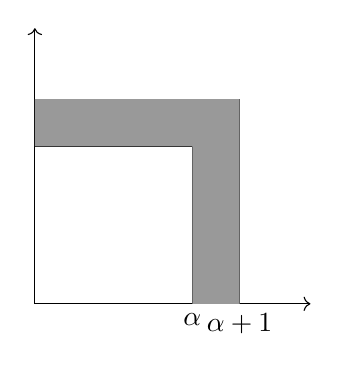
\begin{tikzpicture}
\draw[->] (0,0) -- (3.5,0);
\draw[->] (0,0) -- (0,3.5);
\draw (2,0) -- (2,2) -- (0,2);
\draw (2.6,0) -- (2.6,2.6) -- (0,2.6);
\draw (2,0) node [anchor=north] {$\alpha$};
\draw (2.6,0) node [anchor=north] {$\alpha+1$};
\fill[black!40!white] (2,0) -- (2.6,0) -- (2.6,2.6) -- (0,2.6) -- (0,2)
-- (2,2);
\end{tikzpicture}
\end{center}

If \(\gamma_\alpha\le\omega^\alpha\), then
\begin{equation*}
\gamma_{\alpha+1}\le\omega^\alpha+\alpha\cdot 2+1
\end{equation*}
Since \(\alpha\cdot\omega\le\omega^\alpha\), 
\begin{equation*}
\gamma_{\alpha+1}\le\omega^\alpha+\alpha\cdot 2+1\le\omega^\alpha+\alpha\cdot\omega\le
\omega^\alpha\cdot 2\le\omega^{\alpha+1}
\end{equation*}
\end{proof}

\begin{exercise}
There is a well-ordering of the class of all finite sequences of ordinals
s.t. for each \(\alpha\), the set of all finite sequences in \(\omega_\alpha\) is
an initial segment and its order-type is \(\omega_\alpha\)
\end{exercise}

\begin{proof}
We need to show that \(\Gamma(\omega_\alpha^\omega)=\omega_\alpha\), which is
to show \(\Gamma(\omega_\alpha^n)=\omega_\alpha\) for any \(n\in\omega\).
\end{proof}

We say that a set \(B\) is a \emph{projection} of a set \(A\) if there is a mapping of
\(A\) onto \(B\). Note that \(B\) is a projection of \(A\) if and only if there is a
partition \(P\) of \(A\) such that \(\abs{P}=\abs{B}\). If \(\abs{A}\ge\abs{B}>0\),
then \(B\) is a projection of \(A\). Conversely using the Axiom of Choice, one
shows that if \(B\) is a projection of \(A\), then \(\abs{A}\ge\abs{B}\). This
cannot be proved without the Axiom of Choice

\begin{exercise}
The set of all finite subsets of \(\omega_\alpha\) has cardinality \(\aleph_\alpha\)
\end{exercise}

\begin{exercise}
\(\omega_{\alpha+1}\) is a projection of \(P(\omega_\alpha)\)
\end{exercise}
\begin{proof}
Consider \(f:P(\omega_\alpha\times\omega_\alpha)\to\omega_{\alpha+1}\). If
\(R\subset\omega_\alpha\times\omega_\alpha\) is a well-ordering, let
\(f(R)=\type(R)\) and \(f(\omega_\alpha\times\omega_\alpha)=\omega_\alpha\)
\end{proof}
\begin{exercise}
\(\aleph_{\alpha+1}<2^{2^{\aleph_\alpha}}\)
\end{exercise}
\begin{proof}
\(\aleph_{\alpha+1}\) is a projection of \(P(\aleph_\alpha)\). Hence
\begin{equation*}
\aleph_{\alpha+1}<2^{\aleph_{\alpha+1}}\le 2^{2^{\aleph_\alpha}}
\end{equation*}
\end{proof}
\begin{exercise}[$\zf$]
Show that \(\omega_2\) is not a countable union of countable sets.
\end{exercise}
\begin{proof}
Assume that
\end{proof}
\section{Real Numbers}
\label{sec:org6204848}
The set of all real numbers \(\R\) (the \emph{real line} or the \emph{continuum}) is the
unique ordered field in which every nonempty bounded set has a least upper bound.
\begin{theorem}[Cantor]
The set of all real numbers is uncountable
\end{theorem}
\begin{proof}
Let us assume that the set \(\R\) of all reals is countable, and let
\(c_0,\dots,c_n,n\in\N\) be an enumeration of \(\R\).

Let \(a_0=c_0\) and \(b_0=c_{k_0}\) where \(k_0\) is the least \(k\) s.t. \(a_0<c_k\).
For each \(n\), let \(a_{n+1}=c_{i_n}\), where \(i_n\) is the least \(i\) s.t.
\(a_n<c_i<b_n\), and \(b_{n+1}=c_{k_n}\) where \(k_n\) is the least \(k\) s.t.
\(a_{n+1}<c_k<b_n\). If we let \(a=\sup\{a_n:n\in\N\}\), then \(a\neq c_k\) for all \(k\)
\end{proof}

\subsection{The Cardinality of the Continuum}
\label{sec:org2e69f92}
Let \(\fc\) denote the cardinality of \(\R\). As the set \(\Q\) of all rational
numbers is dense in \(\R\), every real number \(r\) is equal to
\(\sup\{q\in\Q:q<r\}\) and because \(\Q\) is countable, it follows that
\(\fc\le\abs{P(\Q)}=2^{\aleph_0}\) 

Let \(\bC\) (the \emph{Cantor Set}) be the set of all reals of the form 
\(\sum_{n=1}^\infty a_n/3^n\) where each \(a_n=0\) or 2. \(\bC\) is obtained by
removing from the closed interval \([0,1]\). \(\bC\) is in a one-to-one
correspondence with the set all \(\omega\)-sequences of 0's and 2's and so
\(\abs{\bC}=2^{\aleph_0}\)

Therefore \(\fc\ge 2^{\aleph_0}\) and so by the Cantor-Berstein Theorem we have
\begin{equation*}
\fc=2^{\aleph_0}
\end{equation*}

In \(\zfc\) every infinite cardinal is an aleph and so
\(2^{\aleph_0}\ge\aleph_1\). Cantor's conjecture then becomes the statement 
\begin{equation*}
2^{\aleph_0}=\aleph_1
\end{equation*}
known as the \emph{Continuum Hypothesis} (CH).
\subsection{The Ordering of \(\R\)}
\label{sec:orge52300f}
A linear ordering \((P,<)\) is \emph{complete} if every nonempty boudned subset of \(P\)
has a least upper bound.

\begin{definition}[]
A lienar ordering \((P,<)\) is \emph{dense} if for all \(a<b\) there exists a \(c\) s.t.
\(a<c<b\)

A set \(D\subset P\) is a \emph{dense subset} if for all \(a<b\) in \(P\) there exists a
\(d\in D\) s.t. \(a<d<b\).

An ordered set is \emph{unbounded} if it has neither a least nor a greatest element
\end{definition}

\begin{theorem}[Cantor]
\begin{enumerate}
\item Any two countable unbounded dense linearly ordered sets are isomorphic
\item \((\R,<)\) is the unique complete linear ordering that has a countable dense
subset isomorphic to \((\Q,<)\)
\end{enumerate}
\end{theorem}
\begin{proof}
\begin{enumerate}
\item Let \(P_1=\{a_n:n\in\N\}\) and \(P_2=\{b_n:n\in\N\}\) be two such linearly ordered
sets. We construct an isomorphism \(f:P_1\to P_2\) in the following way: we
first define \(f(a_0)\), then \(f^{-1}(b_0)\), then \(f(a_1)\), then \(f^{-1}(b_1)\),
etc., so as to keep \(f\) order-preserving. For example, to define \(f(a_n)\), if
it's not yet defined, we let \(f(a_n)=b_k\) where \(k\) is the least index s.t.
\(f\) remains order-preserving (such a \(k\) always exists because \(f\) has been
defined for only finitely many \(a\in P_1\))
\item To prove the uniqueness of \(\R\), let \(C\) and \(C'\) be two complete dense
unbounded linearly ordered sets, let \(P\) and \(P'\) be dense in \(C\) and
\(C'\), respectively, and let \(f\) be an isomorphism of \(P\) onto \(P'\). Then
\(f\) can be extended to an isomorphism \(f^*\) of \(C\) and \(C'\): For \(x\in C\)
let \(f^*(C)=\sup\{f(p):p\in P\text{ and }p\le x\}\)
\end{enumerate}
\end{proof}

The existence of \((\R,<)\) is proved by means of \textbf{Dedekind cuts} in \((\Q,<)\).
The following theorem is a general version of this construction:

\begin{theorem}[]
Let \((P,<)\) be a dense unbounded linearly ordered set. Then there is a
complete unbounded linearly ordered set \((C,\prec)\) s.t.
\begin{enumerate}
\item \(P\subset C\) and \(<\) and \(\prec\) agree on \(P\)
\item \(P\) is dense in \(C\)
\end{enumerate}
\end{theorem}
\begin{proof}
A \textbf{Dedekind cut} in \(P\) is a pair \((A,B)\) of disjoint nonempty subsets of \(P\)
s.t.
\begin{enumerate}
\item \(A\cup B=P\)
\item \(a<b\) for any \(a\in A\) and \(b\in B\)
\item \(A\) does not have a greatest element
\end{enumerate}


Let \(C\) be the set of all Dedekind cuts in \(P\) and let
\((A_1,B_1)\preceq(A_2,B_2)\) if \(A_1\subset A_2\). The set \(C\) is complete: If
\(\{(A_i,B_i):i\in I\}\) is a nonempty bounded subset of \(C\), then
\((\bigcup_{i\in I}A_i,\bigcap_{i\in I}B_i)\) is its supremum.

For \(p\in P\), let
\begin{equation*}
A_p=\{x\in P:x<p\},\quad B_p=\{x\in P:x\ge P\}
\end{equation*}
Then \(P'=\{(A_p,B_p):p\in P\}\) is isomorphic to \(P\) and is dense in \(C\)
\end{proof}
\subsection{Suslin's Problem}
\label{sec:org9018a19}
The real line is, up to isomorphism, the unique linearly ordered set that is
dense, unbounded, complete and contains a countable dense subset.

Since \(\Q\) is dense in \(\R\), every nonempty open interval of \(\bR\) contains
a rational number. Hence if \(S\) is a disjoint collection of open intervals,
\(S\) is at most countable. (\(f:S\to\Q\) is injective)

Let \(P\) be a dense linearly ordered set. If every disjoint collection of open
intervals in \(P\) is at most countable, then we say that \(P\) satisfies the
\textbf{countable} \textbf{chain condition}

\emph{\textbf{Suslin's Problem}. Let \(P\) be a complete dense unbounded linearly ordered}
\emph{set that satisfies the countable chain condition. Is \(P\) isomorphic to the}
\emph{real line?}

This question cannot be decided in \(\zfc\)
\subsection{The Topology of the Real Line}
\label{sec:org6865bb4}
The real line is a metric space with the metric \(d(a,b)=\abs{a-b}\). Its
metric topology coincides with the order topology of \((\R,<)\). Since \(\Q\) is
a dense set in \(\R\) and since every Cauchy sequence of real numbers
converges, \(\R\) is a separable complete metric space. (A metric space is
\textbf{separable} if it has a countable dense set; it is \textbf{complete} if every Cauchy
sequence converges)

Every open sets is the union of open intervals with rational endpoints.\footnote{Check \href{https://math.stackexchange.com/questions/318299/any-open-subset-of-bbb-r-is-a-at-most-countable-union-of-disjoint-open-interv}{StackExchange}} 

Every open interval has cardinality \(\fc\)

A nonempty closed set is \textbf{perfect} if it has no isolated points.

\begin{theorem}[]
Every perfect set has cardinality \(\fc\)
\end{theorem}

\begin{proof}
Given a perfect set \(P\), we want to find a one-to-one function
\(F:\{0,1\}^\omega\hookrightarrow P\). Let \(S\) be the set of all fintie
sequences of 0's and 1's. By induction on the length of \(s\in S\) one can
fined closed intervals \(I_s\) s.t. for each \(n\) and all \(s\in S\) of length of
\(n\),
\begin{enumerate}
\item \(I_s\cap P\)
\item the diameter of \(I_s\) is \(\le 1/n\)
\item \(I_{s^\frown 0}\subset I_s,I_{s^\frown 1}\subset I_s\) and
\(I_{s^\frown 0}\cap I_{s^\frown 1}=\emptyset\)
\end{enumerate}



For each \(f\in\{0,1\}^\omega\), the set 
\(P\cap\bigcap_{n=0}^\infty I_{f\restriction n}\) has exactly one element
\end{proof}

\begin{theorem}[Cantor-Bendixson]
If \(F\) is an uncountable closed set then \(F=P\cup S\) where \(P\) is perfect and
\(S\) is at most countable
\end{theorem}
\begin{corollary}[]
If \(F\) is a closed set, then either \(\abs{F}\le\aleph_0\) or
\(\abs{F}=2^{\aleph_0}\)
\end{corollary}
\begin{proof}
For every \(A\subset\R\), let
\begin{equation*}
A'=\text{the set of all limit points of } A
\end{equation*}
\(A'\) is closed, and if \(A\) is closed then \(A'\subset A\). Thus we let
\begin{align*}
&F_0=F,\quad F_{\alpha+1}=F_\alpha'\\
&F_\alpha=\displaystyle\bigcap_{\gamma<\alpha}F_\gamma\text{ if }\alpha>0
\text{ is a limit ordinal} 
\end{align*}
Since \(F_0\supset F_1\supset\dots\supset F_\alpha\supset\dots\), there exists
an ordinal \(\theta\) s.t. \(F_\alpha=F_\theta\) for all \(\alpha\ge\theta\). We let
\(P=F_\theta\) 

If \(P\) is nonempty, then \(P'=P\) and so it's perfect. Thus the proof is
completed by showing that \(F-P\) is at most countable.

Let \(\la J_k:k\in\N\ra\) be an enumeration of rational intervals. We have
\(F-P=\bigcup_{\alpha<\theta}(F_\alpha-F_\alpha')\); hence if \(a\in F-P\), then
there is a unique \(\alpha\) s.t. \(a\) is an isolated point of \(F_\alpha\). We let
\(k(a)\) be the least \(k\) s.t. \(a\) is the only opoint of \(F_\alpha\) in the
interval \(J_k\). Note that if \(\alpha\le\beta\), \(b\neq a\) and \(b\in
   F_\beta-F_\beta'\), then \(b\not\in J_{k(a)}\). Thus the correspondence
\(a\mapsto k(a)\) is one-to-one
\end{proof}
A set of reals is called \textbf{nowhere dense} if its closure has empty interior.

\begin{theorem}[The Baire Category Theorem]
If \(D_0,D_1,\dots,D_n,\dots,n\in\N\) are dense open sets of reals, then the
intersection \(D=\bigcap_{n=0}^\infty D_n\) is dense in \(\R\)
\end{theorem}
\subsection{Borel Sets}
\label{sec:org14e6af3}
\begin{definition}[]
An \textbf{algebra of sets} is a collection of \(\cals\) of subsets of a given set \(S\)
s.t.
\begin{enumerate}
\item \(S\in\cals\)
\item if \(X\in\cals\) and \(Y\in\cals\) then \(X\cup Y\in\cals\)
\item if \(X\in\cals\) then \(S-X\in\cals\)
\end{enumerate}


A \textbf{\(\sigma\)-algebra} is additionally closed under countable unions (and
intersections)
\begin{enumerate}
\setcounter{enumi}{3}
\item if \(X_n\in\cals\) for all \(n\), then \(\bigcup_{n=0}^\infty X_n\in\cals\)
\end{enumerate}
\end{definition}

\begin{definition}[]
A set of reals \(B\) is \textbf{Borel} if it belongs to the smallest \(\sigma\)-algebra
\(\calb\) of sets of reals that contains all open sets.
\end{definition}
\end{document}